\documentclass[12pt,a4paper]{scrartcl}
\usepackage[ngerman, english]{babel}
\usepackage[T1]{fontenc}
\usepackage[utf8]{inputenc}
\usepackage[color=yellow!15]{todonotes}
\usepackage{graphicx}
\usepackage[numbers, sort&compress, square]{natbib}
\usepackage[colorlinks, linkcolor=black, citecolor=blue, urlcolor=blue]{hyperref}
\usepackage{titlesec}
\usepackage{color}

% used for line numbering
\usepackage{lineno}

% The following parameters seem to provide a reasonable page setup.
\topmargin -1.0cm
\oddsidemargin 0.2cm
\textwidth 15cm 
\textheight 23cm
\footskip 1.0cm


%The next command sets up an environment for the abstract to your paper.
\newenvironment{sciabstract}{%
\begin{quote} \bfseries}
{\end{quote}}


% If your reference list includes text notes as well as references,
% include the following line; otherwise, comment it out.

\renewcommand\refname{References and Notes}

% The following lines set up an environment for the last note in the
% reference list, which commonly includes acknowledgments of funding,
% help, etc.  It's intended for users of BibTeX or the {thebibliography}
% environment.  Users who are hand-coding their references at the end
% using a list environment such as {enumerate} can simply add another
% item at the end, and it will be numbered automatically.

\newcounter{lastnote}
\newenvironment{scilastnote}{%
\setcounter{lastnote}{\value{enumiv}}%
\addtocounter{lastnote}{+1}%
\begin{list}%
{\arabic{lastnote}.}
{\setlength{\leftmargin}{.22in}}
{\setlength{\labelsep}{.5em}}}
{\end{list}}


% Include your paper's title here

\title{\textbf{ \Large{Reducing data traffic in wireless structural health monitoring systems using embedded computing}}}


\author
{Katrin Jahr, Robert Schlich\\
\\
\normalsize{Degree program “Civil Engineering” (M.Sc.)}\\
\normalsize{Bauhaus-Universität Weimar, Germany}\\
\\
\normalsize{katrin.jahr@uni-weimar.de}\\
\normalsize{robert.schlich@uni-weimar.de}
}


% Include the date command, but leave its argument blank.
\date{}



%%%%%%%%%%%%%%%%% END OF PREAMBLE %%%%%%%%%%%%%%%%



\begin{document} 

% Double-space the manuscript.

\baselineskip18pt

% Make the title.

\maketitle 

% 
%\sloppy
\setlength{\emergencystretch}{3pt}
\hyphenation{sample-rate auto-nomous moni-toring}

\begin{sciabstract}

The dependability and accuracy of wireless structural health monitoring systems can be affected by data loss during wireless data transmission.
Applying adequate data compression methods can significantly reduce the amount of data that has to be transmitted and lower the occurrence of data loss.
In this paper, the design and implementation of a wireless structural health monitoring system, capable of data compression is presented. 
A fast Fourier transform is used on every sensor node to analyze oscillation frequencies. 
Only the first natural frequency of the oscillation and the correlated magnitude are transmitted to the base station.
In laboratory experiments, devised to validate the proposed approach, the data traffic is reduced by xx %.

\end{sciabstract}

%----------------------------------------------------------------------------------------

\linenumbers % Schaltet Zeilennummerierung ein
\modulolinenumbers[5] % nur jede 5. Zeile

\section*{Dictionary}

\begin{tabular}{|l|l|}
\hline 
Sensorknoten (SunSPOT) & sensor node \\ 
\hline 
einzelner Messsensor (Thermometer) & sensor \\ 
\hline 
Knoten im neuronalen Netz & neuron \\ 
\hline 
eine abgeschlossene Messungreihe & test run \\ 
\hline 
gemessene Werte & sensor data \\ 
\hline 
vorhergesagte Werte & predicted data \\ 
\hline 
durch Vorhersage erwartete Werte & expected data \\ 
\hline 
einzelner Messwert & measurement \\ 
\hline 
Test & laboratory experiments\\ 
\hline
tatsächliche, nicht virtuelle Messung & actual measurement \\
\hline
Messaufbau & test setup \\
\hline
\end{tabular} 

%----------------------------------------------------------------------------------------

\section*{Introduction}

Civil engineering structures are exposed to various external impacts during their lifetime. 
Structural health monitoring (SHM) systems can be deployed to evaluate the conditions and to ensure the structural stability of civil engineering structures.
\citet{BisbySHM} defines SHM as "a non-destructive \textit{in-situ} structural evaluation method that uses any of several sensors which are attached to, or embedded in, a structure".
The obtained sensor data is collected by sensor nodes, and then analyzed and stored on a computer system over long periods of time. 
The analysis of the sensor data can reveal abnormal changes in material and geometric behaviour at an early stage.

Traditionally, the sensor nodes are connected to computer systems with cables.
Using wired SHM systems has several disadvantages, including expensive wiring, high installation and labor costs as well as inaccessibility of optimal sensor location with wires.
In wireless SHM systems, the sensor nodes communicate---through a basestation with each other and with computer systems--- via wireless transceivers, eradicating wiring-specific problems.

However, when using wireless SHM systems, special attention has to be paid to data transfer.
Immense amounts of raw data incure and have to be transmitted.
Over the air transmission is error-prone and may lead to irreparable data loss.  (klingt das zu stark? Warum ist das mit FFT nicht mehr so schlimm?)
To save transmission time and storage space, and to decrease data loss, the transmidded data can be reduced using embedded computing.
Depending on the measuring objective, first steps of data processing can be conducted decentralized directly on the sensor nodes.
Transmitting analysis results instead of raw data can reduce the amount of transmitted data exponentially.

In this paper, the natural frequency of a building structure is determined using a fast Fourier transform.
Deviations from the natural frequency indicate changes in the vibration behavior, which may be caused by structural failures.

%\begin{itemize}
%	\item problem: viel data traffic
%	\item daten können verloren gehen
%	\item lösung: embedded computing, decentralized data analysis on sensor nodes 
%	\item fft
%\end{itemize}

This paper is organized as follows:
First, a wireless structural health monitoring system is designed and implemented. 
Next, a decentralized data analysis approach, using fast Fourier transform, is developed.
Then, the system is tested in laboratory experiments.
Finally, the experimental results are discussed and future research directions are proposed.

%----------------------------------------------------------------------------------------

\section*{Design and implementation of the wireless structural health monitoring system}
In the following section, the wireless structural health monitoring system is introduced and the software implementation is described.
The wireless SHM system consists of wireless sensor nodes and a host computer, linked with a basestation.
The sensor nodes and the basestation are of type "Oracle Sun SPOT". 
The Sun SPOTS are equipped with several components, see \autoref{fig:SPOT}.
Among others, the sensor board includes an accelerometer and eight independent RGB-LEDs.
The 3-axis digital output accelerometer with sensitivity ranging between $\pm$\,2\,g and $\pm$\,8\,g has a maximum sampling rate of 125Hz \citep{eDemo2010}.

\begin{figure}[ht]
    \centering
    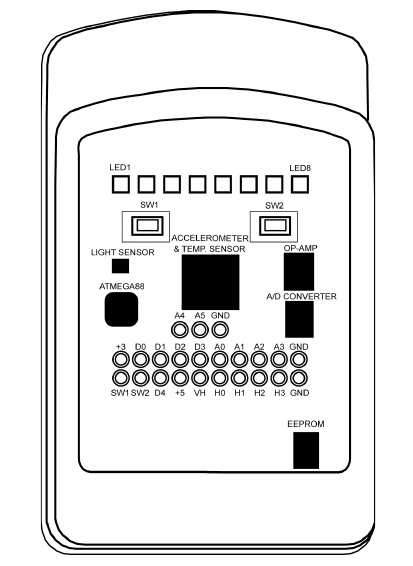
\includegraphics[scale=0.5]{figures/eDemoboard.png}
    \caption{Layout of the Sun SPOT sensor board \cite{spotToO}}
    \label{fig:SPOT}
\end{figure}

The SHM system performs the following tasks:
1. data acquisition,
2. data processing,
3. data transmission, 
4. data storage,
5. diagnostics and 
6. information retrieval.
Tasks 1 to 3 are executed by the sensor nodes: During system operation, the sensor nodes acquire acceleration measurements and perform a fast Fourier transform to determine the characteristics of the oscillation of the structure. 
The processed data is then transmitted via radio to the basestation and, finally, to the host computer.
On the host computer, tasks 4 is conducted by storing the data in a MySQL database.
Task 5 and 6---additional analysis and diagnosis---are conducted on the host computer in further steps.

\colorbox{cyan}{neuer Absatz:}

The SHM system is programmed object-oriented in Java. 
Object orientation uses objects which are instanciated using classes as paradigm. 
A class includes methods, allowing the objects to perform actions, and attributes, storing object-specific data.
The SHM system consists of two packages---\texttt{sensornode} and \texttt{basestation}.
A package organizes several Java classes that build a program.

\autoref{fig:UML-sn} describes the classes of the \texttt{sensor\-node} package.
The package \texttt{sensor\-node} consists of the classes \texttt{Acceleration\-Sampler}, \texttt{FFT}, \texttt{Communi\-cation} and \texttt{Main\-Spot}, which are embedded directly into the sensor nodes.
The \texttt{Acceleration\-Sampler} class is responsible for measuring the acceleration.
There are two phases: \colorbox{cyan}{At} first, the acceleration is measured with a low sampling rate.
Once the acceleration exceeds a threshold, the \colorbox{cyan}{second phase is entered} by increasing the sampling rate. 
The measured values are stored into an array.
The different phases are indicatad by lighting different LEDs.
The \texttt{FFT} class performs a fast Fourier transform on the measured accelerations. 
With the transformed data, the magnitudes and the correlating frequencies of the measured oscillation are calculated.
Finally, the natural frequency \colorbox{cyan}{is} determined by extracting the maximal magnitude.
The \texttt{Communi\-cation} class opens a radio connection between the sensor node and the basestation to transfer data from the sensor node to the basestation.
For starting the operation of \colorbox{cyan}{the sensor node}, the entry point of the programm is the \texttt{start\-App()} method in the \texttt{Main\-Spot} class. 
Within the \texttt{Main\-Spot} class, instances of the \texttt{Acceleration\-Sampler} class, the \texttt{FFT} class and the \texttt{Communication} class are created to perform the measurement.

\begin{figure}[ht]
    \centering
    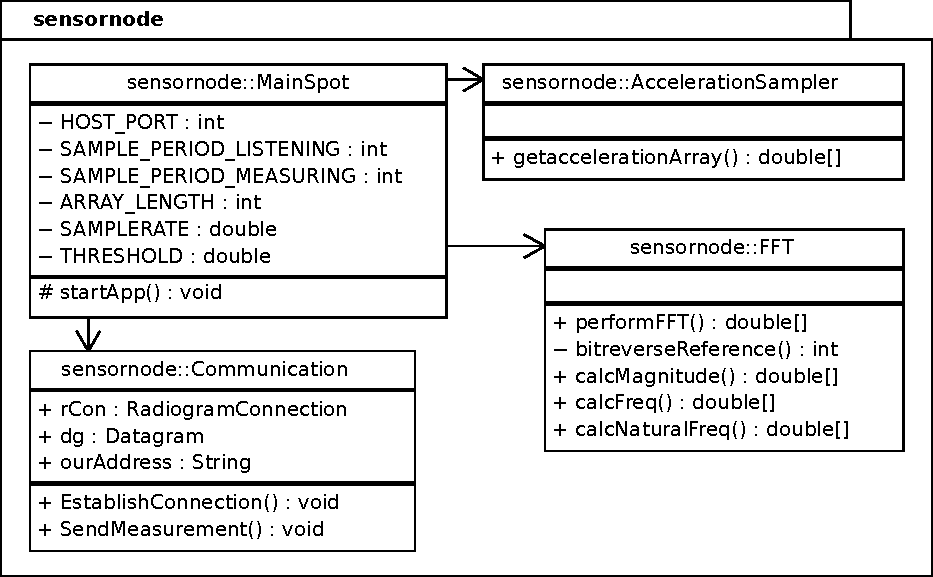
\includegraphics[width = \textwidth]{figures/uml-sensornode.pdf}
    \caption{class diagram of the sensornode package}
    \label{fig:UML-sn}
\end{figure}

\autoref{fig:UML-bs} describes the classes of the \texttt{base\-station} package.
The package \texttt{base\-station} runs on the host computer and operates the basestation.
It consists of the classes \texttt{Database\-Handler} and \texttt{Main\-Base}.

The \texttt{Database\-Handler} class establishes a connection to a MySQL database, creates a database table, if none with the specified name is available, and inserts data into the database table.
The entry point of the program is the \texttt{run()} method in the \texttt{Main\-Base} class. The \texttt{Main\-Base} class opens a radio connection between the basestation and the sensor nodes, receives data sent by the sensor nodes and creates an instance of \texttt{Database\-Handler} to insert the data into the database.

\begin{figure}[h!]
    \centering
    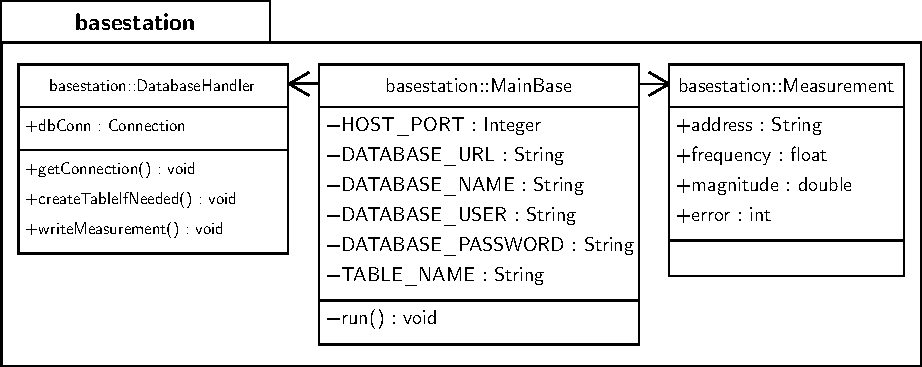
\includegraphics[width = \textwidth]{figures/uml-basestation.pdf}
    \caption{class diagram of the basestation package}
    \label{fig:UML-bs}
\end{figure}

\newpage

%----------------------------------------------------------------------------------------

\section*{Laboratory experiments}

In the following section, the laboratory experiments are described.
First a describtion of the test setup is given, second, the data aquisition and processing are depicted, and finally, the results are discussed. 

To validate the proposed approach in laboratory experiments, the wireless SHM system is installed on a test structure.
The test structure is a 4-story shear-frame consisting of four steel plates of 25\,cm\,$\times$\,50\,cm and a thickness of 0.8\,mm.
The plates are mounted on threaded rods with a vertical clearance of 23\,cm.
At the bottom, the rods are fixed into a solid block of 40\,cm\,$\times$\,60\,cm and a height of 30\,cm.
The SHM system is installed on the test structure by fastening a wireless sensor node to each story.
The laboratory setup after system installation is shown in \autoref{fig:teststructure}.

\todo{Bild ersetzen durch ein Bild mit den fertig installierten SPOTS}

\begin{figure}[h!]
    \centering
    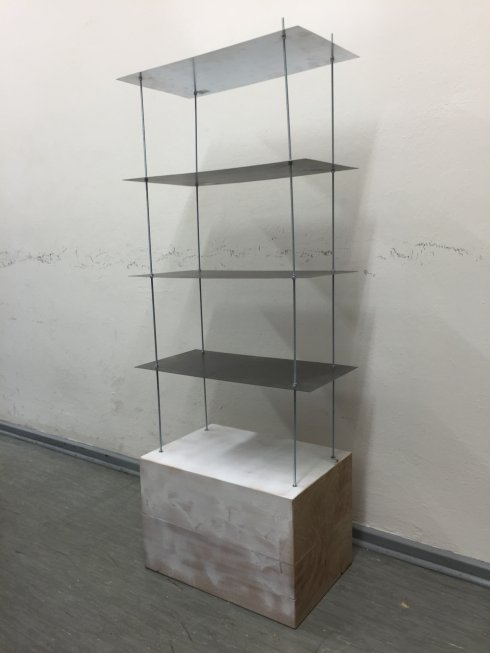
\includegraphics[scale=0.4]{figures/teststructure.jpg}
    \caption{Laboratory setup}
    \label{fig:teststructure}
\end{figure}

The structure is excited by deflecting and releasing the top of the structure.
This excitation method ensures a free vibration in natural frequency with little interferences.
After excitation, the sensor nodes automatically start measuring acceleration with an increased sampling rate of 50\,Hz.
To minimize the wireless data communication, each node performs a fast Fourier transform algorithm once sufficient acceleration measurements have been collected.
The acceleration measurements are converted into the vibration frequencies and the corresponding magnitudes of the building.
Each sensor node transfers only the values of the predominating frequency---i.e. the frequency with the biggest magnitude--- \colorbox{cyan}{to the basestation}. 
The values are then stored in the MySQL database at the host computer.

The correct implementation of the FFT has been verified beforehand by plotting the frequency domain of various oscillation events.
\autoref{fig:fft-diagram} shows  one of the results as an example.
The natural frequencies are readily identifiable by the peaks in the diagram.
The first three natural frequencies are located at approximately 2.3\,Hz (first natural frequency), 8\,Hz (second natural frequency),and 16\,Hz (third natural frequency).
The same natural frequencies appeared throughout repeated tests with varying excitation forces, sampling rates, and number of measurements.

\begin{table}[ht]
	\centering
	\begin{tabular}{c c c}
		1\textsuperscript{st} natural frequency & 2\textsuperscript{nd} natural frequency & 3\textsuperscript{rd} natural frequency \\ 
		2,3 & 8 & 16 \\
	\end{tabular}
	\caption{Natural frequencies of the test structure}
	\label{tab:nat-freqs}
\end{table}

\begin{itemize}
	\item 
	\item that means our paper is also wireless and very very good
\end{itemize}

%----------------------------------------------------------------------------------------

\section*{Summary}

\begin{itemize}
	\item data traffic was reduced by XX\,\% 
\end{itemize}

%----------------------------------------------------------------------------------------

\bibliographystyle{unsrtnat}
\bibliography{literature}

\end{document}
